%!TEX root = emnlp2016.tex

\section{Model Validation with Simulated Data}
\label{sec:valid}

Before using Capsule to explore a corpus of real messages (described
in \cref{sec:eval}), we provide a quantitative validation of the model
using simulated data.

We used the generative process in \cref{fig:generative-model} to
create ten data sets, each with 100 time intervals, ten general
topics, ten entities, and roughly 20,000 messages. We then used these
data sets to compare Capsule's event detection performance to that of
four baseline methods. We also compared the methods' abilities to
identify the most relevant messages for each event.

\subsection{Detecting Events}
\label{sec:detecting_events}

For each data set, we ordered the time intervals from most to least
eventful, using the ``eventness'' measure described in
\cref{sec:detecting} and the simulated values of the latent
variables. We then treated these ranked lists of time intervals as
``ground truth'' and assessed how well each method was able to recover
them.

For Capsule itself, we used our approximate inference algorithm to
obtain a fitted variational distribution for each simulated data
set. We then ordered the time intervals using our ``eventness''
measure and the posterior expected values of the latent variables.

For our first baseline, we constructed an ``event-only'' version of
Capsule by dropping the first and second terms in
\cref{eq:poisrate}. We used this baseline to test whether modeling
``business as usual'' discussion makes it easier to detect significant
events. We obtained a fitted variational distribution for this model
using a variant of our approximate inference algorithm, and then
ordered the time intervals using our ``eventness'' measure, modified
appropriately, and the posterior expected values of the latent variables.

For our second baseline, we drew inspiration from previous work on
event detection in the context of news articles, and focused on each
time interval's deviation in term counts from the
average. Specifically, we ordered the time intervals $1, \ldots, T$
for each simulated data set according to this measure:
\begin{equation}
  \sum_{v=1}^V \sum_{\substack{d=1\\t_d \!=\! t}}^D \left\lvert n_{dv} - \frac{1}{D}\sum_{d=1}^D
  n_{dv} \right\rvert.
\label{eq:wordev}
\end{equation}

We added tf-idf term weights for our third baseline:
\begin{equation}
  \sum_{v=1}^V \textrm{tf-idf}\,(v)
  \sum_{\substack{d=1\\t_d\!=\!t}}^D \left\lvert n_{dv} - \frac{1}{D}\sum_{d=1}^D
  n_{dv} \right\rvert.
\label{eq:tfidfwordev}
\end{equation}

Finally, we randomly ordered the time intervals for each data set to
serve as a straw-man baseline.

We also experimented with baselines that involved term-count
deviations on the entity level and topic-usage deviations on the
message level~\cite{dou2012leadline}, but found that they were not
competitive.

For each data set, we compared each method's ranked list of time
intervals to the corresponding ``ground-truth'' list of time
intervals, by dividing the sum of the lists' actual set overlap at
each rank by the sum of their maximum set overlap at each rank:
\begin{equation}
\frac{\sum_{r=1}^T \vert S^{\textrm{truth}}_r \cap
  S^{\textrm{method}}_r \vert}{\sum_{r=1}^T r},
\label{eq:detection}
\end{equation}
where $S^{\textrm{truth}}_r$ is a set of the top $r$ time intervals
according to the ``ground-truth'' list and $S^{\textrm{method}}_r$ is
a set of the top $r$ time intervals according to the method.

\begin{figure}[t]
\centering
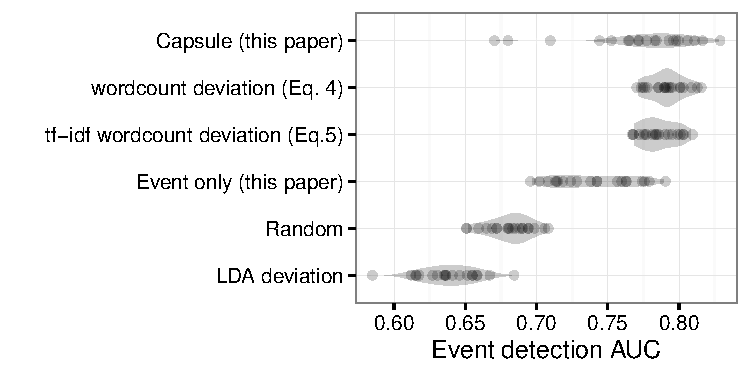
\includegraphics[width=\linewidth]{fig/sim_eventdetect.pdf}
\caption{Event detection performance using ten simulated data
  sets. Each dot represents the performance (\cref{eq:detection};
  higher is better) of a single method on a single data set; each
  shaded green area summarizes the distribution of performance for a
  single method.  Capsule outperforms all four baseline methods.}
\label{fig:sim_eventdetect}
\end{figure}


\Cref{fig:sim_eventdetect} shows that Capsule outperforms all four
baseline methods. These results serve as a sanity check for both the
model and its implementation.

%\footnote{The model was set with the same
%  number of topics $K=10$ and exponential decay $f$ used to simulate
%  the data.  More details on the decay function surround its formal
%  definition in \cref{eq:f}.}

\subsection{Identifying Relevant Messages}

For each data set, we created a list of the most relevant messages for
each time interval $t$ by computing $f(t_d, t)\,\epsilon_{dt}$ for
each message $d$ (using the simulated values of $\epsilon_{dt}$) and
ordering the messages accordingly. We then treated these ranked lists
of messages as ``ground truth'' and assessed how well Capsule and the
baseline methods were able to recover them.

For Capsule, we used our approximate inference algorithm to obtain a
fitted variational distribution for each data set, and then, for each
time interval, ordered the messages according to $m_{dt} = f(t_d,
t)\,\E[\epsilon_{dt}]$. For our second and third baselines, we ordered
the messages sent during each time interval according message-specific
versions of \cref{eq:wordev,eq:tfidfwordev}.
%---i.e.,
%\begin{equation}
%  \sum_{v=1}^V \left\lvert n_{dv} - \frac{1}{D}\sum_{d=1}^D
%  n_{dv} \right\rvert
%\end{equation}
%and
%\begin{equation}
%  \sum_{v=1}^V \textrm{tf-idf}\,(v) \left\lvert n_{dv} - \frac{1}{D}\sum_{d=1}%^D
%  n_{dv} \right\rvert.
%\end{equation}

For each data set, we compared each method's ranked list of messages
for each time interval to the corresponding ``ground-truth'' list, by
computing precision at 10 messages. The average precision for Capsule
was was 0.44, while the average precision for the ``event-only''
version of the model was 0.09. The other baselines recovered zero
relevant messages.

\section{Exploratory Analysis}
\label{sec:eval}

Capsule is intended to help analysts explore and understand their
data. In this section, we demonstrate its capabilities by analyzing a
corpus of over two million U.S. State Department cables from the
1970s.

\subsection{Data}

The National Archive collects diplomatic cables sent between the
U.S. State Department and its foreign embassies. We obtained a subset
of this corpus from the Central Foreign Policy Files at the National
Archives, via the History Lab at Columbia
University.\footnote{http://history-lab.org} The subset contains over
two million cables sent between 1973 and 1978. In addition to the text
of the cables, each message is labeled with its author (e.g., the
U.S. State Department, a particular embassy, or a named individual),
its recipients (often several), and the date the cable was sent. We
used a vocabulary of 6,293 terms and omitted cables with fewer than
three terms, resulting in 2,021,852 cables sent between 22,961
entities. We used weekly time intervals, as few cables were sent on
the weekends.

\subsection{Model Settings}

We ran our approximate inference algorithm for Capsule to obtain a
fitted variational distribution. We used $K=100$ general topics, the
exponential decay function in \cref{eq:f} with $\tau=4$, and top-level
hyperparameters $s=r=0.3$. With these settings, a single iteration of
the algorithm took about an hour.\footnote{Each iteration of our
  algorithm considers all messages. Modifying it to stochastically
  sample the data would reduce the time required to obtain an
  equivalent fitted variational distribution.}

\subsection{Detecting Well-Known Events}

To evaluate Capsule's ability to detect well-known events, we used a
list, provided to us by the History Lab, of thirty-nine well-known
events that took place between 1973 and 1978. Each event is present in
at least one of six reputable collections of historic events, such as
the Office of the Historian's Milestones in the History of
U.S. Foreign
Relations.\footnote{\url{https://history.state.gov/milestones/1969-1976}}
We treated this list of events as ``ground truth'' and assessed how
well Capsule and each of the baselines described in
\cref{sec:detecting_events} were able to recover them.

Specifically, we used each method to construct a ranked list of time
intervals. Then, for each method, we computed the discounted
cumulative gain (DCG), which, in this context, is equivalent to
computing
\begin{equation}
  \sum_{e=1}^{39} \frac{1}{\log{\left(\textrm{rank}\left(e, L_T^{\textrm{method}}\right)\right)}},
\end{equation}
where $L_T^{\textrm{method}}$ is the method's ranked list of time
intervals and $\textrm{rank}\left(e, L_T^{\textrm{method}}\right)$ is
the rank of the $e^{\textrm{th}}$ well-known event in
$L_T^{\textrm{method}}$. Finally, we divided the DCG by the ideal
DCG---i.e., $\sum_{e=1}^{39} \frac{1}{\log{\left(e\right)}}$---to
obtain the normalized DCG (nDCG). \Cref{table:cables:ndcg} shows that
Capsule outperforms all four baseline methods.

\begin{table}[t]
\centering
\small
\begin{tabular}{cc}
\toprule
\textbf{Method} & \textbf{nDCG} \\
\midrule
Capsule (this paper) & 0.693 \\
term count deviation + tf-idf (\cref{eq:tfidfwordev}) & 0.652 \\
term count deviation (\cref{eq:wordev}) & 0.642 \\
random & 0.557\\
``event-only'' Capsule (this paper) & 0.426\\
\bottomrule
\end{tabular}
\caption{Event detection performance (nDCG; higher is better) using
  thirty-nine well-known events that took place between 1973 and 1978.
  Capsule outperforms all four baseline methods.}
\label{table:cables:ndcg}
\end{table}

%Additionally, we computed held-out validation data likelihood on the model and each of its component parts; \Cref{table:cables:ll} shows that the full Capsule model captures the data better than any of its component parts individually.
%\begin{table}[bt]
%\centering
%\begin{tabular}{l c c}
%\toprule
%\textbf{Model} & \textbf{LL, 10 iter.} & \textbf{LL, final} \\
%\midrule
%Full Capsule & -1.62e7 & -1.52e7 \\
%Entity Topics Only & -1.64e7 & -- \\
%General Topics Only & -1.71e7 & -1.53e7 \\
%Event Only & -1.79e7 & -- \\
%\bottomrule
%\end{tabular}
%\caption{Log likelihood (LL) computed on validation data at 10 iterations and at convergence---the event only and entity only models are small enough that they converge with very few iterations. The full Capsule model achieves the lowest log likelihood in both cases.}
%\label{table:cables:ll}
%\end{table}

\subsection{Exploration}

We now turn to our primary goal---using Capsule to explore and
understand a corpus of messages. \Cref{fig:cables_events} shows our
``eventness'' measure (\cref{eq:eventness}) over time. One of the
tallest peaks occurs during the week of December 1, 1975, when the
United Nations General Assembly discussed omnibus decolonization. As
described in \cref{sec:detecting}, we can characterize this event by
computing $m_{dt} = f(t_d, t)\,\E[\epsilon_{dt}]$ for each message $d$
and then ordering the messages accordingly. \Cref{tab:decol} lists the
highest-ranked messages.

\begin{table*}[tb]
\small
\centering
\begin{tabular}{cccc}
\toprule
$f(t_d, t)\, \E[\epsilon_{dt}]$ & \textbf{Date} & \textbf{Author Entity} & \textbf{Subject} \\
\midrule
4.60 & 1975-12-05 & Canberra & 30th UNGA: Item 23, Guam, Obmibus Decolonization and ... \\
4.26 & 1975-12-05 & Mexico & 30th UNGA-Item 23: Guam, Omnibus Decolonization and ... \\
4.21 & 1975-12-06 & State & 30th UNGA-Item 23: Guam, Omnibus Decolonization and ... \\
4.11 & 1975-12-03 & Dakar & 30th UNGA: Resolutions on American Samoa, Guam and ...\\
4.08 & 1975-12-04 & Monrovia & 30th UNGA: Item 23: Resolutions on decolonization and A...\\
\bottomrule
\end{tabular}
\caption{Highest-ranked messages for the week of December 1, 1975,
  when the United Nations General Assembly discussed
  decolonization. Capsule accurately recovers messages related to this
  real-world event. Typos are intentionally copied from the data.}
\label{tab:decol}
\end{table*}

\begin{table*}[ht]
\small
\centering
\begin{tabular}{cccc}
\toprule
$f(t_d, t)\, \E[\epsilon_{dt}]$ & \textbf{Date} & \textbf{Author Entity} & \textbf{Subject} \\
\midrule
5.06 & 1975-05-15 & Sofia & Seizure of US merchant vessel by Cambodian forces \\
5.05 & 1975-05-15 & Dar es Salaam & Seizure of U.S.~merchant vessel by Cambodian forces \\
4.92 & 1975-05-16 & Lusaka & Seizure of US merchant vessel by Cambodian forces \\
4.61 & 1975-05-13 & Zagreb & Waiver request for INS Vienna visas Eagle name check... \\
4.59 & 1975-05-15 & State & eizure of US merchant Vessel by Cambodian forces \\
\bottomrule
\end{tabular}
\caption{Highest-ranked messages for the week of May 12, 1975, when the
  S.S.~Mayaguez, an American merchant vessel, was captured. Capsule
  accurately recovers messages related to this real-world event. Typos
  are intentionally copied from the data.}
\label{tab:mayaguez}
\end{table*}

Another notable event was the seizure of the S.S.~Mayaguez, an
American merchant vessel, during May, 1975, at the end of the Vietnam
War. \Cref{tab:mayaguez} lists the highest-ranked messages for this
event. We can examine these messages to confirm their relevancy and
learn more about the event. For example, here is the content of the
most relevant message:
\begin{shaded*} \tt{In absence of MFA Chief of Eighth Department Avramov, I
informed American desk officer Yankov of circumstances surrounding seizure
and recovery of merchant ship Mayaguez and its crew.  Yankov promised to
inform the Foreign Minister of US statement today  (May 15).
Batjer
}
\end{shaded*}


A third week of interest occurs in early July, 1976.  On July 4th, the
US celebrated its Bicentennial, but on the same day, Israeli forces
completed a hostage rescue mission because an Air France flight from
Tel Aviv had been hijacked and taken to Entebbe,
Uganda.\footnote{Capsule assumes that only one event occurs during
  each time interval. This example is a clear violation of this
  assumption, but also serves to demonstrate that Capsule can
  successfully detect and characterize multiple events, even when they
  overlap.} This event was mostly discussed the week after the event
took place; the most relevant messages are listed in
\cref{sec:additional_results} (\cref{tab:entebbe}). The cable from
Stockholm describing the ``Ugandan role in Air France hijacking''
begins with the following content, which reveals further information
about this event:
\begin{shaded*} \tt{
1. We provided MFA Director of Political Affairs
Leifland with Evidence of Ugandan assistance to
hijackers contained in Ref A.  After reading material,{}
Leifland described it a ``quite good'', and said it{}
would be helpful for meeting MFA has scheduled for
early this morning to determine position GOS will take
at July 8 UNSC consideration of Israeli Rescue Operation. ...
}
\end{shaded*}

In addition to detecting and characterizing well-known events, such
the S.S.~Mayaguez incident and Operation Entebbe, Capsule can detect
and characterize more obscure, but potentially significant,
events. For example, the kidnapping of Tenneco employees in 1974 and
Operation Fluid Drive in 1976, both of which appear in
\cref{fig:cables_events}, were previously unknown to our expert
historian at the History Lab. Capsule's analysis also reveals that
the United Nations held a Security Council meeting in Panama during
1973---our expert historian did not previously know that the United
Nations had held any meetings in this country.

Capsule also provides a way to explore ``business-as-usual''
discussion using the posterior expected values of the general topics
$\mathbold{\beta}_1, \ldots, \mathbold{\beta}_K$ and the entity topics
$\mathbold{\eta}_1, \ldots, \mathbold{\eta}_A$. Examples of each of
these types of topics are in \cref{sec:additional_results}
(\cref{tab:topics,tab:entities}, respectively); these examples
illustrate that, as desired, the entity topics absorb
location-specific terms, preventing them from overwhelming the general
topics.

